\section{Realization}
%Focus generale sulle tecnologie utilizzate
In this section we outline the technical aspects concerning the realization of our framework. Therefore we first discuss presents the enabler technologies through which we instantiate the design principles presented in \cref{sec:design}. After that, we discuss the interaction workflow between the instantiated technologies. Finally we show implementation details.
\begin{figure}[t]
\centering
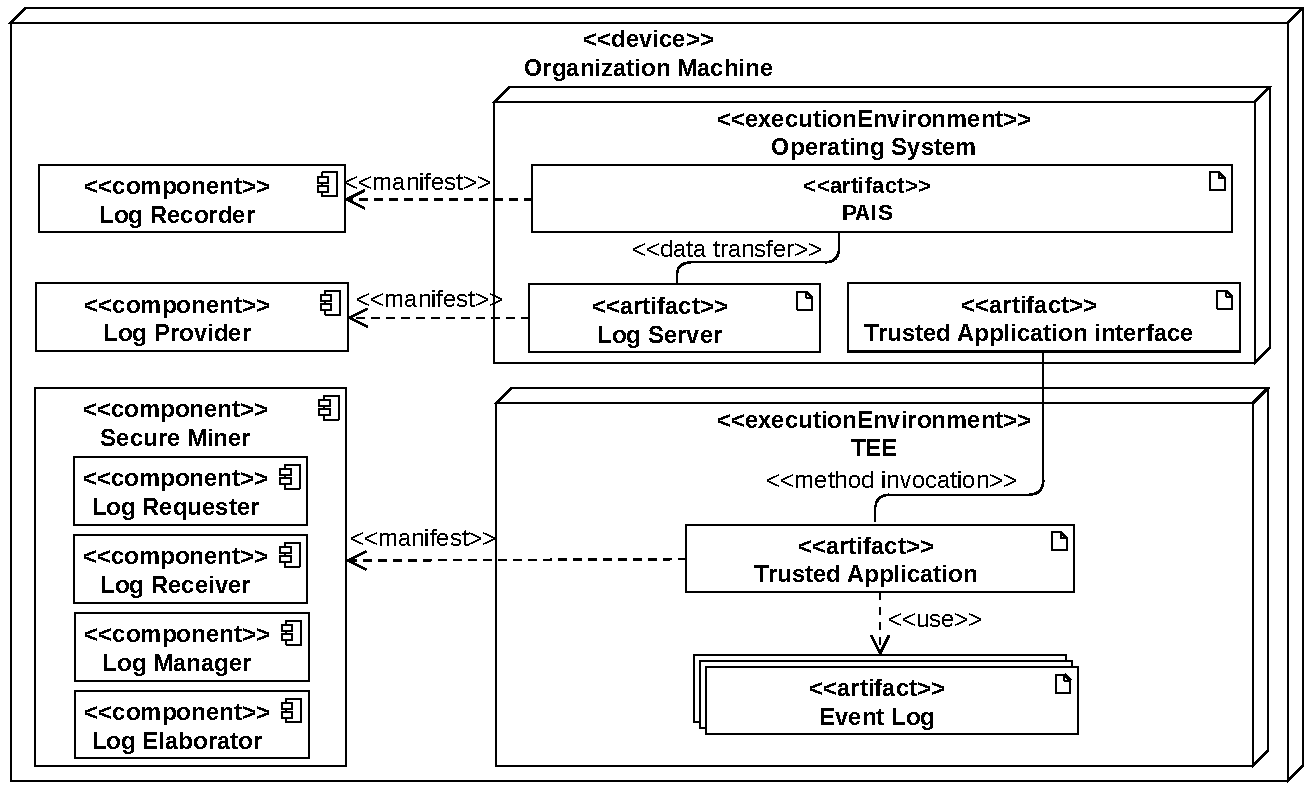
\includegraphics[width=11cm]{content/figures/deployment_diagram.pdf}
\caption{UML deployment diagram.}
\label{fig:deployment_diagram}
\end{figure}
\subsection{Deployment}

\subsection{Workflow}
\subsection{Implementation}
%\subsubsection{Event Log Generation}
%Tecnologie utilizzate
%Sintesi del processo di generazione dei log
%\subsubsection{Trusted Miner and Log Provider}
%Tecnologia TEE usata
%Linguaggio usato per programmare in TEE
%Algoritmo implementato
%Rappresentazioni intermedie (PNML, Petrinet, ecc...)
%Linguaggio Log provider
